\documentclass[11pt, a4paper]{report}
\usepackage[utf8]{inputenc} % Required for inserting images
\usepackage[skip=10pt plus1pt, indent=0pt]{parskip}
\usepackage{mathpazo}%font type
\usepackage{domitian}%font type
\usepackage[T1]{fontenc}%font type
\usepackage[czech]{babel}
\usepackage{amssymb}
\usepackage{fancyhdr}
\usepackage{graphicx}
\usepackage{xcolor}
\usepackage{geometry}
\usepackage{subcaption}
\usepackage{algpseudocode} 
\usepackage{algorithm}
\usepackage{algorithmicx}

\usepackage{floatrow}
\usepackage{amsmath} % matice

\usepackage{hyperref}

\usepackage{amssymb} %navííííc, pak vymazat

\graphicspath{ {./images} }
\geometry{a4paper, left=20mm, right=20mm, bottom=20mm, top=15mm}

\begin{document}
%edit title page
\begin{titlepage}
    \centering
        {\bfseries\Large
            UNIVERZITA KARLOVA\\
            PŘÍRODOVĚDECKÁ FAKULTA\\
            \vskip2cm
        } 
        \vfill
             
\includegraphics[width=7cm]{logo_natur} % also works with logo.pdf
        \vfill
        {\bfseries\Large
            \vskip2cm
            {\Large ALGORITMY POČÍTAČOVÉ KARTOGRAFIE\par}
            \vskip0.3cm
            Digitální modely terénu\\
            \vskip4.5cm
        }
\vfill
    {\large\raggedleft Daniela DANČEJOVÁ, \\Anna KOŽÍŠKOVÁ, \\Praha 2023\par} 
\vfill
\vfill
\end{titlepage}

% insert  each sections
\chapter*{Zadání}

\par\emph{Vstup: Souvislá polygonová mapa n polygonů} \{$P_1, ..., P_n$\}, \emph{analyzovaný bod q}.
\par \emph{Výstup: $P_i, q \in P_i$}.

\par Nad polygonovou mapou implementujte Ray Crossing Algorithm pro geometrické vyhledání incidujícího polygonu obsahujícího zadaný bod \emph{q}.
\par Nalezený polygon graficky zvýrazněte vhodným způsobem (např. vyplněním, šrafováním, blikáním). Grafické rozhraní vytvořte s využitím frameworku QT.
\par Pro generování nekonvexních polygonů můžete navrhnout vlastní algoritmus či použít existující geografická data (např. mapa evropských států).
\par Polygony budou načítány z textového souboru ve Vámi zvoleném formátu. Pro datovou reprezentaci jednotlivých polygonů použijte špagetový model.
\bigbreak

% insert table
\par\textbf{\large Hodnocení:}
\bigbreak
\begin{center}
    \begin{tabular}{|p{14.2cm}|c|} 
     \hline\large
         \textbf{Krok} & \textbf{Hodnocení}\\ %[0.5ex] 
             \hline\hline
             \small Detekce polohy bodu rozlišující stavy uvnitř, vně polygonu. & \small10b \\ 
             \hline
             \emph{\small Analýza polohy bodu (uvnitř/vně) metodou Winding Number Algorithm.} & \emph{\small +10b} \\
             \hline
             \emph{\small Ošetření singulárního případu u Winding Number Algorithm: bod leží na hraně polygonu.} & \emph{\small +5b} \\
             \hline
             \emph{\small Ošetření singulárního případu u Ray Crossing Algorithm: bod leží na hraně polygonu.} & \emph{\small +5b} \\
             \hline
             \emph{\small Ošetření singulárního případu u obou algoritmů: bod je totožný s vrcholem jednoho či více polygonů.} & \emph{\small +2b}\\ 
             \hline
             \emph{\small Zvýraznění všech polygonů pro oba výše uvedené singulární případy.} & \emph{\small +3b}\\  
             \hline
             \textbf{Max celkem:} & \textbf{35b}\\ %[0.3ex] 
             \hline
    \end{tabular}
\end{center}
\chapter*{Popis a rozbor problému }

\par Často řešenou úlohou v oblasti počítačové grafiky a digitální kartografie bývá určování vzájemného vztahu polohy daného bodu a uzavřené oblasti (Bayer 2008). Řešení tohoto úkolu, známého jako \emph{Point-in-Polygon Problem} (PIPP), poskytuje informaci o tom, zda se bod nachází uvnitř, vně nebo na hranici souvislého uzavřeného útvaru (polygonu). Možnosti řešení se pro konvexní a nekonvexní útvary liší zejména v náročnosti algoritmů potřebných pro zohlednění specifických případů polohy vrcholů jednotlivých polygonů (Rourke 2005). Bayer (2023) rozlišuje 2 základní techniky řešení PIPP:

\begin{itemize}
  \item převedení problému na vztah bodu a mnohoúhelníku; 
  \item planární dělení roviny.
\end{itemize}

\par V prvním případě jde o opakované určování polohy bodu vzhledem k mnohoúhelníku; tato technika je snadno implementovatelná, avšak pomalejší. V druhém případě je rovina rozdělena na množinu pásů či lichoběžníků, čímž vzniká \emph{trapezoidální mapa} (Rourke 2005). Rozdělení rovin vede k rychlejšímu nalezení řešení, implementace však bývá obtížnější.
\par Zjištění vzájemné polohy bodu a konvexního útvaru je možné provést jednoduchými algoritmy, například testováním polohy bodu vůči každé hraně útvaru (tzv. \textbf{\emph{Half-plane test}}, složitost \emph{O}(\emph{n})). Nacházejí uplatnění především v triangulačních algoritmech. Mnoho takových algoritmů však nelze použít samo o sobě pro nekonvexní útvary, které se často vyskytují právě v oblasti geoinformatiky a kartografie.
\par Existují dva základní algoritmy vhodné pro nekonvexní útvary schopny detekovat vzájemnou polohu bodu a uzavřené oblasti: \textbf{\emph{Winding Number Algorithm}} a \textbf{\emph{Ray Algorithm}}. Oba tyto algoritmy mají časovou složitost \emph{O}(\emph{n}), přičemž jeden z nich je výrazně rychlejší (Rourke 2005). Těmto algoritmům bude níže věnována samostatná pozornost.

\bigbreak

\section*{Winding Number Algorithm}
\par Winding Number algoritmus je prvním z řešení, kterým lze analyzovat polohu bodu pro nekonvexní mnohoúhelníky. V české literatuře se může označovat jako metoda \emph{ovíjení}. Algoritmus je založen na sčítání/odečítání úhlů, který svírá bod s jednotlivými segmenty polygonu. Za předpokladu, že součet úhlů je \emph{2$\pi$}, pak se bod nachází uvnitř polygonu. Segmentem je uvažována přímka tvořená dvěma po sobě následujícími body v polygonu.
\par Zjednodušeně řečeno, bude-li se pozorovatel dívat z bodu do každého vrcholu v polygonu a bude postupně sčítat úhly, o které se otáčí, součet výsledného úhlu bude 360° (Bayer 2008, Žára 2004).

%\newpage

\par {\large\textbf{Podstata algoritmu} }
\par Mějme uzavřenou oblast \emph{O} v $\mathbb{R}^2$, jejíž hrany tvoří množinou bodů \emph{P} = {$\{P_1, ..., P_n, P_1$\} a bod {\emph{q}}}. Výsledná hodnota algoritmu Winding Number je součet všech uhlů, které opíše průvodič v polygonu. \newline Platí vztah:

\begin{equation}\Omega = \sum_{i=1}^{n} \omega_i.\end{equation}

\par Aby bylo možné spočítat celkový úhel pro daný polygon, je nejprve nutné analyzovat polohu bodu \emph{q} vůči každé přímce, která je definovaná dvěma po sobě následujícími vrcholy $p_i$ a $p_{i+1}$ jež tvoří segment v polygonu. Vzájemná poloha bodu a dané přímky  se vyšetří pomocí Half-plane testu, kde mohou nastat 3 situace (Bayer 2023):

\begin{itemize}
  \item bod q leží vpravo od přímky,
  \item bod q leží vlevo od přímky,
  \item bod q leží na přímce.
\end{itemize}

\par Jako testovací kritérium se použije vztah pro výpočet determinantu matice, která se skládá z vektorů $\vec{p} = (p_x,p_y)$ a $\vec{s} = (s_x,s_y)$:

\begin{equation}\begin{aligned}\vec{p} = p_{i+1} - p_i, \\
 \vec{s} = q - p_i.\end{aligned}\end{equation}

\par Vztah pro výpočet determinantu:
\begin{equation}det = (p_x*s_y)-(s_x*p_y).\end{equation}

\par Pokud
\begin{equation} det\begin{cases} < 0, & \text{bod\emph{ q}\ leží vpravo od přímky} \\ > 0,& \text{bod }q\text{ leží vlevo od přímky} \\ = 0 , & \text{bod }q\text{ leží na přímce} \end{cases}\end{equation}

\par Následně je potřeba procházet jednotlivé hrany v polygonu a sčítat, či odečítat všechny úhly $\omega_i + \omega_{i+1} + ... + \omega_n$ ve směru hodinových ručiečk (nebo v opačném směru) v závislosti na výsledku determinantu. Pro výpočet úhlu $\omega$ je nutné spočíst vektory $\vec{u} = (u_x,u_y)$ a $\vec{v} = (v_x,v_y)$ spočtené jako (viz obrázek 1): 

\begin{equation}\begin{aligned}\vec{u} = p_i - q, \\
                                \vec{v} = p_{i+1} - q .
 \end{aligned}\end{equation}

\begin{figure}[h]
    \centering
        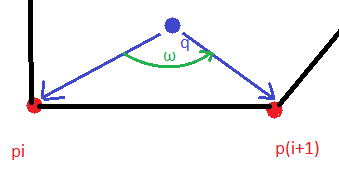
\includegraphics[width=7cm]{uhel} % also works with logo.pdf
    \caption{Úhel vektorů $\vec{u}$ a $\vec{v}$}
\end{figure}

\newpage

\par Velikost úhlu se pak spočítá podle vztahu:
\begin{equation}\cos(\omega) = \frac{\vec{u}\cdot\vec{v}}{||\vec{u}||\cdot||\vec{v}||}\end{equation}

\par Pro následující kroky je nutné pracovat s absolutní hodnotou úhlu $\omega$, jelikož se bude v dalším kroku rozhodovat o jeho přičtení, nebo odečtení.
\begin{equation}|\omega| = \arccos\left(\frac{\vec{u}\cdot\vec{v}}{||\vec{u}||\cdot||\vec{v}||}\right)\end{equation}

\par Bude-li
\begin{equation} det\begin{cases} < 0, & \text{{ pak }$-=\omega$} \\ > 0,& \text{{ pak }$+=\omega$} \end{cases}\end{equation}

\par Následně se všechny úhly sečtou podle vztahu (1) a pokud:
\begin{equation} \Omega\begin{cases} = 2\pi, & \text{\emph{q}}\ \in O, \\ < 2\pi,& \text{\emph{q}} \ \notin O. \\\end{cases}\end{equation}

\par {\large\textbf{Speciální případy algoritmu} }
\par Takto výše popsaný algoritmus bude schopný detekovat bod uvnitř polygonu a mimo něj. Následující část bude věnována případu, kdy se bude analyzovaný bod \emph{q} nacházet na hraně polygonu. Vztah (4) se již částečně o tomto případu zmiňuje. Bod bude ležet na hraně právě tehdy, když
\begin{equation}det = 0.\end{equation}

\par Pro následnou implementaci však pouze tato podmínka nestačí, a proto se dále dá detekovat bod na hraně právě tehdy, když
\begin{equation}\omega = \pi.\end{equation}

\par Výše uvedené dva vztahy ovšem nezohledňují situaci, kdy se bod bude nacházet v jednom z vrcholů množiny \emph{P}. Pro ošetření této možnosti se využije podmínky:
\begin{equation}\text{if\emph{ q}} = p_i\end{equation}
pak se bod nachází ve vrcholu - tedy na hraně polygonu.

\vfill
\par {\large\textbf{Pseudokód} }
\par Na závěr této sekce jsou výše zmíněné kroky shrnuty v pseudokódu, který je implementován v metodě \emph{windingNumberAlgorithm} v souboru \emph{algorithms.py}.
\vfill

\begin{algorithm}[h]
\caption{ Winding Number}\label{alg:cap}
\begin{algorithmic}
\Require $q: bod, pol: polygon$
\Ensure $-1 ,0 ,1$
\State $n \gets {\text{\emph{délka polygonu}}}$
\State $eps \gets {\text{\emph{prahová hodnota}}}$ \Comment{velmi malá kladná hodnota blízká 0}
\State $totalAngle \gets 0$ \Comment{inicializace velikosti úhlu}
\For{všechny vrcholy v polygonu}
    \If{bod je vrchol} 
    \State {\text{\textbf{vrať} hodnotu -1}}\Comment{bod leží na hraně}
    \EndIf

    \State {\text{Spočti vektor \emph{p}:} pi+1 - i}
    \State {\text{Spočti vektor \emph{s}:} q - pi}
    \State {\text{Spočti determinant z vektorů \emph{p} a \emph{s}}}
    \State {\text{Spočti vektor \emph{u}:} pi - q}
    \State {\text{Spočti vektor \emph{v}:} pi+1 - q}
    \State {\text{Spočti úhel $\omega$ z vektorů \emph{u} a \emph{v}}}

    \If{determinant je větší než 0} 
        \State $totalAngle \gets +{\text{$\omega$}}$
    \ElsIf{determinant je menší než 0}
        \State $totalAngle \gets -{\text{$\omega$}}$
    \EndIf
    \If{determinant je 0 a zároveň je úhel (\emph{u} a \emph{v}) - $\pi$ menší než eps} 
        \State {\text{\textbf{vrať} hodnotu -1}} \Comment{bod leží na hraně}
    \EndIf
\EndFor
\If{absolutní hodnota( z (abs. hodnoty totalAngle)) - 2$\pi$ je menší než eps}
    \State {\text{\textbf{vrať} hodnotu 1}} \Comment{bod leží uvnitř polygonu}
\Else{} 
    \State {\text{\textbf{vrať} hodnotu 0}} \Comment{bod leží vně polygonu}
\EndIf
\end{algorithmic}
\end{algorithm}

\newpage

\section*{Ray Crossing Algorithm}
\par Další možné řešení PIPP pro nekonvexní útvary představuje \emph{Ray Crossing Algorithm}, který bývá také označován jako \emph{Ray Algorithm}, \emph{Ray Casting Algorithm} nebo \emph{Even-Odd Rule Algorithm}, v češtině i jako \emph{paprskový algoritmus} (Bayer 2008). Tento algoritmus zjišťuje vzájemný vztah polohy bodu a útvaru na základě počtu průsečníků, které tvoří polopřímka vedena z daného bodu s hranami tohoto útvaru. V případě, že je tento počet lichý, uvažovaný bod se nachází uvnitř polygonu, je –li tento počet sudý nebo rovný nule, uvažovaný bod se nachází vně polygonu. V případě, že je s uvažovaným bodem totožný právě jeden průsečík, tento bod se nachází na hraně polygonu (obrázek 2).

\begin{figure}[h]
\centering

\includegraphics[width=8cm]{raycrossing} % also works with logo.pdf
    \caption{Detekce polohy bodů vzhledem k polygonu za použití Ray Crossing algoritmu (převzato z Rourke 2005, s. 240)}
\end{figure}

\par Tento algoritmus je možné dále modifikovat tak, abychom jeho implementaci zjednodušili a zabránili vzniku problematických situací.

\bigbreak

\par {\large\textbf{Podstata algoritmu} }
\par Mějme uzavřenou oblast \emph{O} v $\mathbb{R}^2$, jejíž hrany tvoří množinou bodů \emph{P} = {$\{P_1, ..., P_n, P_1$\} a bod {\emph{q}}}. Uvažujme vodorovnou testovací přímku \emph{r} procházející bodem \emph{q} takovou, že 
\begin{equation} r(q): y=y_q.\end{equation}

\par Počet průsečíku \emph{k} přímky \emph{r} s oblastí \emph{O} pak určuje polohu bodu \emph{q} vůči \emph{O} tak, že
\begin{equation} k\%2=\begin{cases} 1, & \text{\emph{q}}\ \in O, \\ 0 , & \text{\emph{q}} \ \notin O. \\\end{cases}\end{equation}

\par Tato varianta algoritmu však neřeší případy, když \emph{r}(\emph{q}) prochází vrcholem $P_i$ nebo hranou a neumí detekovat stav, když \emph{q} leží na hraně $\delta$. Pro vylepšení je možné provést modifikaci algoritmu s redukcí ke \emph{q} a rozdělením \emph{r} na dvě polopřímky $r_1$ a $r_2$ s opačnou orientací: nechť je $r_1$ levostranná a $r_2$ pravostranná polopřímka. Udržujme si počet levostranných a pravostranných průsečíků $k_l$ a $k_r$. Zavedeme–li si lokální souřadnicový systém s počátkem v bodě \emph{q} a osami \emph{x'}, \emph{y'} a polopřímky  $r_1(q)$ a $r_2(q)$ ztotožníme s osou \emph{x'} tak, že je možné je popsat rovnicí (Bayer 2023)
\begin{equation} y' = 0,\end{equation}

\par můžeme provést redukci bodů $p_i = [x_i, y_i]$ ke $q$:
\begin{equation}\begin{aligned}x'_i = x_i - x_q, \\
                               y'_i = y_i - y_q.
 \end{aligned}\end{equation}
 
\par Pokud průsečík $M = [x'_m, y'_m = 0]$ segmentu (hrany) oblasti \emph{O} a osy \emph{x'} (jedné z polopřímek \emph{x'}, \emph{y'}) existuje, můžeme ho určit ze vztahu
\begin{equation}x'_m = \frac{x'_{i+1}y'_i - x'_iy'_{i+1}}{y'_{i+1}-y'_i}.\end{equation}

\par Podmínky existence průsečíku $M$ s jednou z polopřímek $r_1(q)$, $r_2(q)$ udávají vztahy:
\begin{itemize}
    \item pro levou polorovinu: 
        \begin{equation} t_l = y_{i+1} < y_q \neq y_i < y_q,\end{equation}
    \item pro pravou polorovinu:
        \begin{equation} t_r = y_{i+1} > y_q \neq y_i > y_q,\end{equation}
\end{itemize}

\par kde $t_l$, $t_r$ nabývají hodnoty \verb|True| nebo \verb|False|. Průsečík $M$ se pak vypočte pro každou polopřímku zvlášť:
\begin{itemize}
    \item pokud $t_l$ = \verb|True| $\land$ $x'_m$ < 0, inkrementujeme $k_l$,
    \item pokud $t_r$ = \verb|True| $\land$ $x'_m$ > 0, inkrementujeme $k_r$.
\end{itemize}

\par Jinak řečeno: Průsečíky pro levou a pravou část budeme započítávat v případě, leží –li počáteční a koncový bod protnutého segmentu v jiné polorovině (vrchní nebo spodní). Pak
\begin{equation} q =\begin{cases} \in \delta $O$, & \text{$k_l\%2 \neq k_r\%2$,} \\ 
    \in \emph{O}, & \text{$k_r\%2 = 1$,} \\ 
    \notin \emph{O}, & \text{jinak.} 
\end{cases}\end{equation}

\par {\large\textbf{Speciální případy algoritmu} }
\par Při řešení PIPP pomocí \emph{Ray Algorithm} může docházet k případům, které je nutno dodatečně ošetřit.
\par Pokud je zvolený bod $q$ totožný s jedním z bodů $p_i$, pak je možné prohlásit, že $q \in \delta O$.
\par Pokud přímka $r(q)$ prochází vrcholem oblasti $O$, může nastat detekce dvou průsečíku (koncový bod jednoho segmentu a počáteční bod druhého segmentu). Situaci je možné ošetřit započtením tohoto vrcholu jako průsečíku jenom jednou (Bayer 2008, Rourke 2005).

\par Pokud platí, že 
\begin{equation}y_{i+1} - y_i = 0,\end{equation}
\par pak body tvoří $p_{i+1}$ a $p_i$ horizontální hranu a výpočet průsečíku ze vztahu (17) nebude možný. Ve vlastní implementaci algoritmu se v tom případě pokračuje následující iterací.
\par Může nastat situace, když se bod $p_i$ chybně zařadí do vrchní nebo spodní poloroviny oblasti $O$, pokud tento bod leží velmi blízko testovací přímky $r(q)$. Je proto vhodné zavést prahovou hodnotu $\varepsilon$, která tento případ ošetří:
\begin{equation}|y_i - y_q| \leq \varepsilon.\end{equation}

\par {\large\textbf{Pseudokód} }
\par Vlastní implementace \emph{Ray Crossing Algorithm} je níže shrnuta v pseudokódu. Nachází se v metodě \emph{rayCrossingAlgorithm} v souboru \emph{algorithms.py}.

\bigbreak

\begin{algorithm}[h]
\caption{ Ray Crossing}\label{alg:cap}
\begin{algorithmic}
\Require $q: bod, pol: polygon$
\Ensure $-1 ,1 ,0$
\State $kr \gets {\text{\emph{počet pravostranných průsečníků}}}$
\State $kl \gets {\text{\emph{počet levostranných průsečníků}}}$ 
\State $n \gets {\text{\emph{délka polygonu}}}$
\For{všechny vrcholy v polygonu}
    \State Spočti $x_i$, $y_i$
    \If{bod je vrchol} \Comment{bod leží na hraně}
    \State {\text{\textbf{vrať} hodnotu -1}}
    \EndIf

    \State Spočti $x_{i+1}, y_{i+1}$
    \If{ ($y_{i+1} - y_i) == 0$} \Comment{horizontální segment}
    \State {\text{\textbf{pokračuj novou iterací}}}
    \EndIf
    \State Spočti průsečník $x'_m$
    \If{ $y_{i+1} < y_q \neq y_i < y_q$} \Comment{spodní segment}
        \If{ $x'_m < 0$} \Comment{průsečník v levé polrovině}
         \State Inkrementuj $k_l$
        \EndIf
    \EndIf
    \If{ $y_{i+1} > y_q \neq y_i > y_q$} \Comment{vrchní segment}
        \If{ $x'_m > 0$} \Comment{průsečník v pravé polrovině}
         \State Inkrementuj $k_r$
        \EndIf
    \EndIf
\EndFor

\If{$k_l\%2 \neq k_r\%2$}
    \State {\text{\textbf{vrať} hodnotu -1}}  \Comment{bod leží na hraně}
\ElsIf{$k_r\%2 = 1$}
    \State {\text{\textbf{vrať} hodnotu 1}}  \Comment{bod leží uvnitř polygonu}
\Else{}
    \State {\text{\textbf{vrať} hodnotu 0}}  \Comment{bod leží vně polygonu}
\EndIf
\end{algorithmic}
\end{algorithm}
\chapter*{Vlastní implementace}

\par Součástí úlohy bylo kromě samotných algoritmů analyzujících polohu bodu v prostoru také vytvoření přívětivého uživatelského prostředí ve frameworku QT, ve kterém je demonstrována funkčnost obou výše zmíněných algoritmů
na zvolené polygonové mapě. 

\section*{Vstupní data}
\par Jako vstupní data byly zvoleny geografická data s kódem \verb|EPSG:5514| (Křovákovo zobrazení). Aplikace umožňuje otevřít, zpracovat a vykreslit prostorové souřadnice pro soubory ve formátu \verb|.JSON| a \verb|.GEOJSON|. K aplikaci jsou přiloženy testovací data v obou formátech v adresáři \emph{/input\textunderscore files/}.
\par Výsledkem analýzy je grafické vykreslení příslušnosti bodu k polygonu, případně k více polygonům v situaci, kdy je bod umístěn na rozhraní dvou nebo více polygonů.

\bigbreak

\section*{Aplikace}
\par Grafické rozhraní aplikace (obrázek 3) bylo vytvořeno v prostředí \verb|Qt Creator 9.0.1| a dále upravováno v prostředí programovacího jazyka \verb|Python 3.11|. Uživateli je umožněno otevřít soubor ve vlastním adresáři a v těle aplikace kliknutím levého tlačítka myši umístit vlastní bod $q$ pro analýzu jeho polohy vůči vstupním datům. 

\begin{figure}[h]
    \centering
        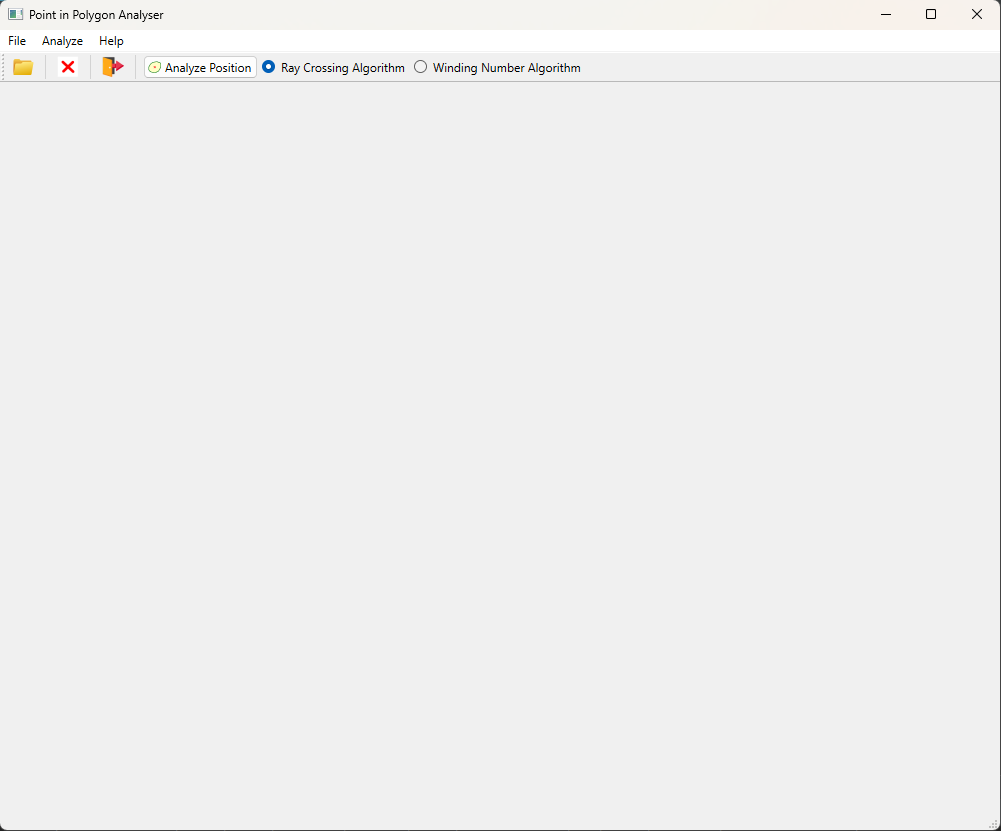
\includegraphics[width=10cm]{aplikace} 
        \caption{Grafické rozhraní aplikace}
\end{figure}

\par Součástí rozhraní je možnost volby matoedy analýzy mezi algoritmy \emph{Ray Crossing} a \emph{Winding Number} (obrázek 4). Po zvolení algoritmu a kliknutí na \verb|Analyze Position| (případně využití klávesové zkratky \verb|Ctrl+A|) se zvýrazní polygon, ve kterém se bod $q$ nachází. V případě, že se bod $q$ nachází na hraně dvou polygonů, resp. na rozhraní více polygonů, zvýrazní se všechny incidující polygony.

\begin{figure}[h]
    \centering
        
\includegraphics[width=10cm]{toolbar} 
        \caption{Panel nástrojů pro volbu algoritmů}
\end{figure}

\par Uživatel má také možnost vstupní polygonovou vrstvu smazat a nahrát novou vrstvu. V případě otevření nového souboru se předešlá vrstva smaže a nahraje se vrstva nová.
\par Vstupní vrstva se nahraje tak, aby vyplnila co nejvíc prostoru v okně aplikace (obrázek 5). S měnící se velikosti okna se ale již nahraná vrstva nemění, je tedy nutno znovu otevřít soubor tak, aby se data vhodně přeškálovala vzhledem k nové velikosti okna. 

\begin{figure}[h]
    \centering
        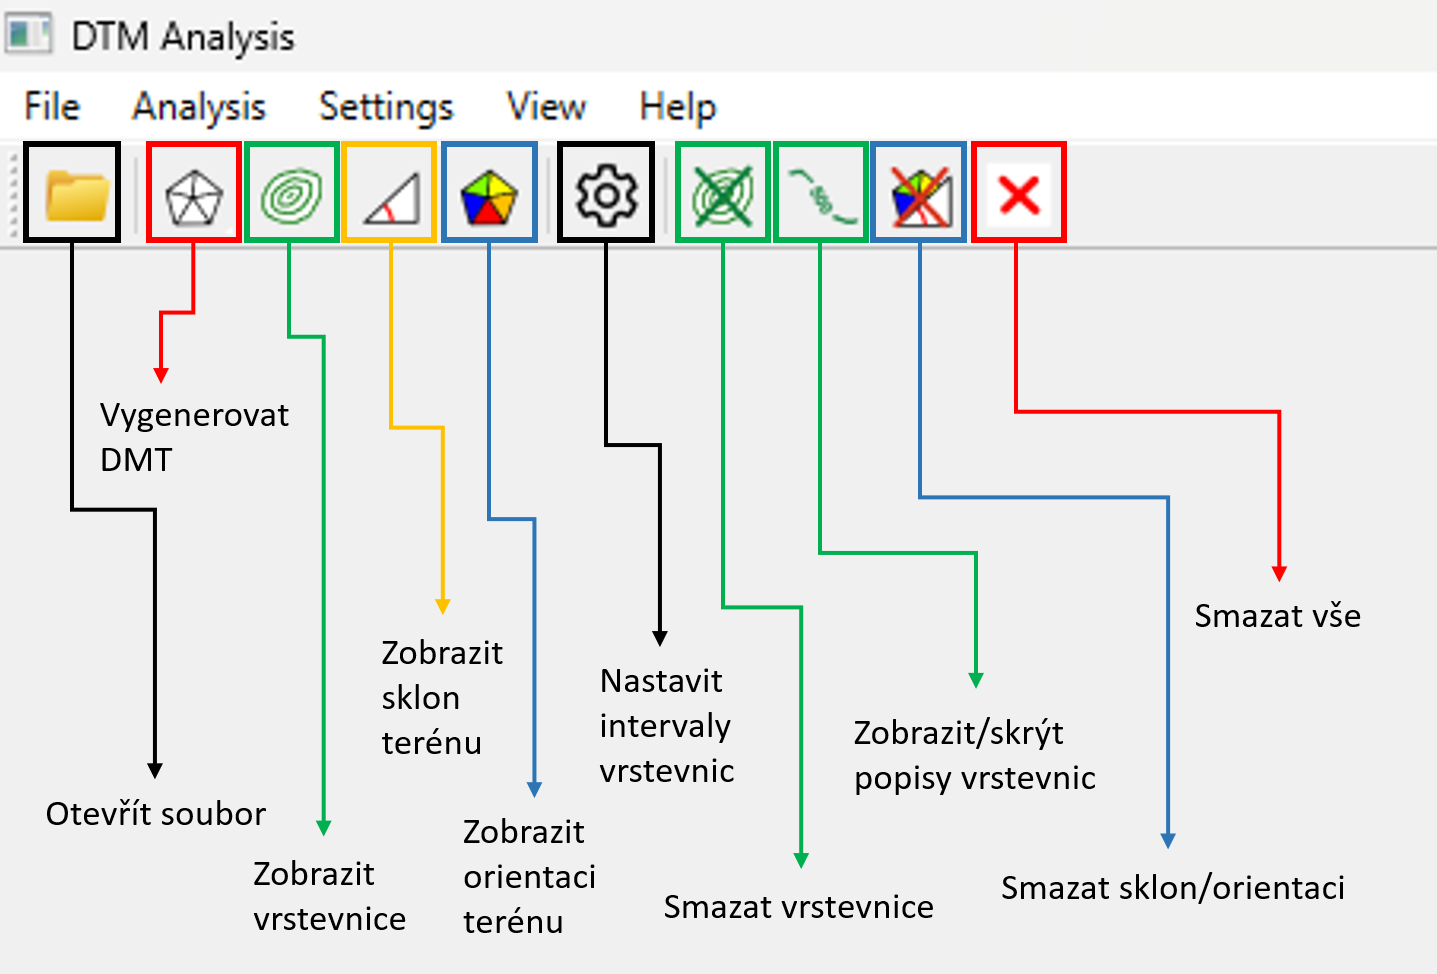
\includegraphics[width=12cm]{showcase} 
        \caption{Ukázka nahrané polygonové vrstvy}
\end{figure}
\par Polygon, ve kterém se zvolený bod může nacházet, se zabarví na modrou barvu. Pokud se zvolený bod nachází na hraně dvou polygonů nebo na vrcholu více polygonů, na tuto skutočnost upozorní vyskakovací okno (obrázek 6) a všechny tyto polygony se zabarví na modrou barvu.

\begin{figure}[h]
    \centering
        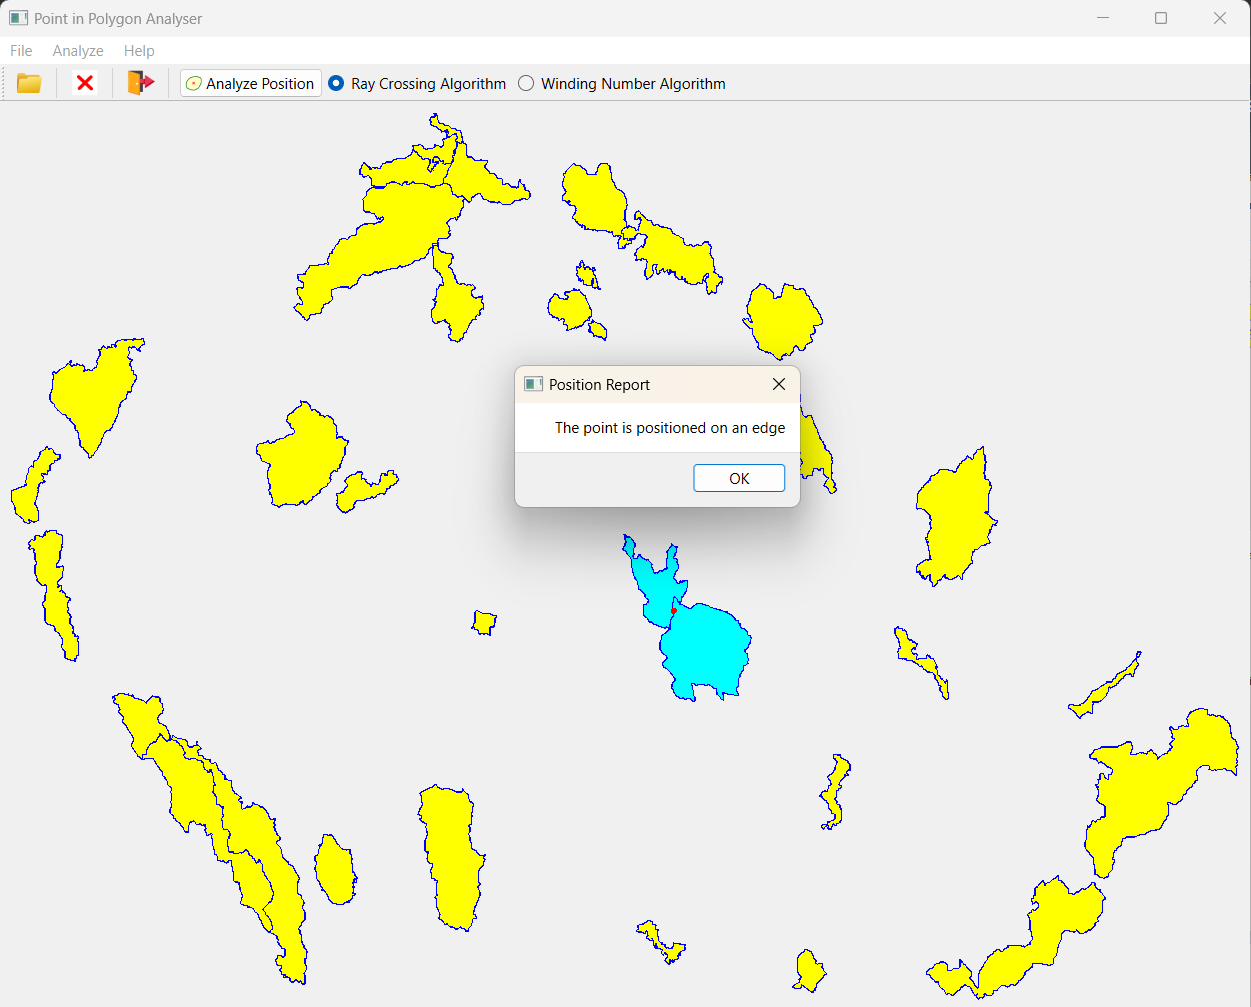
\includegraphics[width=10cm]{highlight} 
        \caption{Vyskakovací okno při detekci hrany}
\end{figure}

\bigbreak

\newpage
\section*{Třídy a metody}
\par Funkční chod aplikace si vyžaduje tři povinné soubory, v kterých jsou implementovány potřebné třídy a metody: \verb|mainform.py|, \verb|algorithms.py| a \verb|draw.py|.

\bigbreak

\par {\large\textbf{Třída MainForm} }
\par Třída MainForm ze souboru \verb|mainform.py| zabezpečuje inicializaci okna aplikace, vrchní lišty, panelu nástrojů, ikon a tlačítek. Zároveň přepojuje jednotlivé interaktivní položky okna s metodami, které vykonají specifické akce. Týkají se především otevření souboru, přepínání algoritmů, provedení analýzy polohy bodu vůči polygonu apod. Část této třídy byla vygenerována v prostředí \verb|Qt Creator 9.0.1| (metody \verb|setupUi()| a \verb|translateUi()|). Níže jsou vyjmenovány nově implementované metody:

\begin{itemize}
    \item \verb|switchToRayCrossing()|
        \subitem{Nastaví algoritmus pro analýzu polohy bodu na \emph{Ray Crossing}.}
    \item \verb|switchToWindingNumber()|
        \subitem{Nastaví algoritmus pro analýzu polohy bodu na \emph{Winding Number}.}
    \item \verb|analyzePosition()|
        \subitem{Provede analýzu polohy bodu $q$ vůči polygonové mapě. Bod a polygonovou mapu (uloženou v seznamu) zavolá z třídy \verb|Draw|. V iteraci přiřadí každému polygonu hodnotu, podle které se polygon zabarví a určí se tak jeho vztah k bodu $q$. Může zavolat metodu pro vyskakovací okno \verb|onEdgePopup()| .}
    \item \verb|processFile()|
        \subitem{Zabezpečuje otevření souboru. Samotný soubor načte do proměnné pomocí metody \verb|openFile()| a následně zavolá metodu \verb|clearEvent()| pro vyprázdnění okna. Pokud je vstupní \verb|JSON| nebo \verb|GeoJSON| nečitelný (např. nestandardní hierarchie položek v slovnících), uživatele na to upozorní vyskakovacím oknem.}
    \item \verb|openFile()|
        \subitem{Otevře \verb|JSON| nebo \verb|GeoJSON| soubor a načte ho do proměnné.}
    \item \verb|exitClick()|
        \subitem{Ukončí aplikaci.}
    \item \verb|clearClick()|
        \subitem{Zavolá metodu \verb|clearEvent()| z třídy \verb|Draw|, která vyprázdní okno.}
    \item \verb|aboutClick()|
        \subitem{Otevře repozitář s aplikací v portálu \verb|GitHub|.}
    \item \verb|onEdgePopup()|
        \subitem{Vytvoří vyskakovací okno v případě, že se zvolený bod nachází na hraně nebo na vrcholu polygonu.}
\end{itemize}

\bigbreak

\par {\large\textbf{Třída Algorithms} }
\par V této třídě jsou obsaženy metody, které byly detailně popsány v předchozí kapitole věnované teorii algoritmů Winding Number a Ray Crossing. Obsahuje metody:

\begin{itemize}
    \item \verb|rayCrossingAlgorithm(q, pol)|,
        \subitem{pro předané parametry \verb|q| (bod) a \verb|pol| (polygon) analyzuje polohu bodu \verb|q| vůči polygonu \verb|pol| pomocí algoritmu Ray Crossing}
    \item \verb|windingNumberAlgorithm(q, pol)|
        \subitem{pro předané parametry \verb|q| (bod) a \verb|pol| (polygon) analyzuje polohu bodu \verb|q| vůči polygonu \verb|pol| pomocí algoritmu Winding Number}
\end{itemize}

\par Třída obsahuje jednu proměnnou \verb|default_alg|, která nastavuje metodu rayCrossingAlgorithm jako primární metodu pro analýzu bodu a polygonu.

\bigbreak

\par {\large\textbf{Třída Draw} }
\par Třída Draw ze souboru \verb|Draw.py| slouží pro inicializaci proměnných nesoucí prostorovou informaci, načítání a vykreslování geoprostorové informace. Při spuštění aplikace se inicializují proměnné pro bod, polygonový list a polygonový status:

\begin{itemize}
  \item \verb|self.__q|,
  \item \verb|self.__polyg_list|,
  \item \verb|self.polyg_status|,
\end{itemize}

\par Třída Draw obsahuje následující metody:
\begin{itemize}
    \item \verb|mousePressEvent(e:QMouseEvent)|
        \subitem{Zodpovídá za změnu pozice bodu.}
    \item \verb|paintEvent(e:QPaintEvent)|
        \subitem{Vykresluje objekty (bod a polygony) na plátno (Canvas).}
    \item \verb|getPoint()|
        \subitem{Vrací souřadnice bodu.}
    \item \verb|getPolygonList()|
        \subitem{Vrací seznam vstupních polygonů.}
    \item \verb|clearEvent()|
        \subitem{Maže vyreslené objekty (bod a polygony) na plátně (Canvas).}
    \item \verb|findBoundingPoints(p:QPointF, xmin, ymin, xmax, ymax)|
        \subitem{Nalezne minimální a maximální souřadnice pro ohraničení polygonu (tzv. bounding box).}
    \item \verb|resizePolygons(xmin, ymin, xmax, ymax)|
        \subitem{Roztáhne vstupní data na plátno podle velikosti okna aplikace.}
    \item \verb|loadData(data)|
        \subitem{Prochází slovník ze vstupního souboru \verb|.JSON/.GEOJSON| a načítá geoprostorovou informaci.}
\end{itemize}

\chapter*{Výsledky}
\par Data \verb|terrain.csv| obsahují celkem 418 trigonometrických bodů z databáze bodových polí ČÚZK (ČÚZK 2023). Body jsou rozmístěny v části Krkonoš a jejich předhůří (obr. 10). Pro analýzu funkčnosti implementovaných metod tvorby DMT byly vybrány tři oblasti se specifickým tvarem reliéfu: 
\begin{enumerate}
    \item oblast s malou vertikální členitostí (rovina, údolí),
    \item oblast s velkou vertikální členitostí (vrcholy, hřbety),
    \item oblast s hřebenem a údolími.
\end{enumerate}

\begin{figure}[H]
\centering
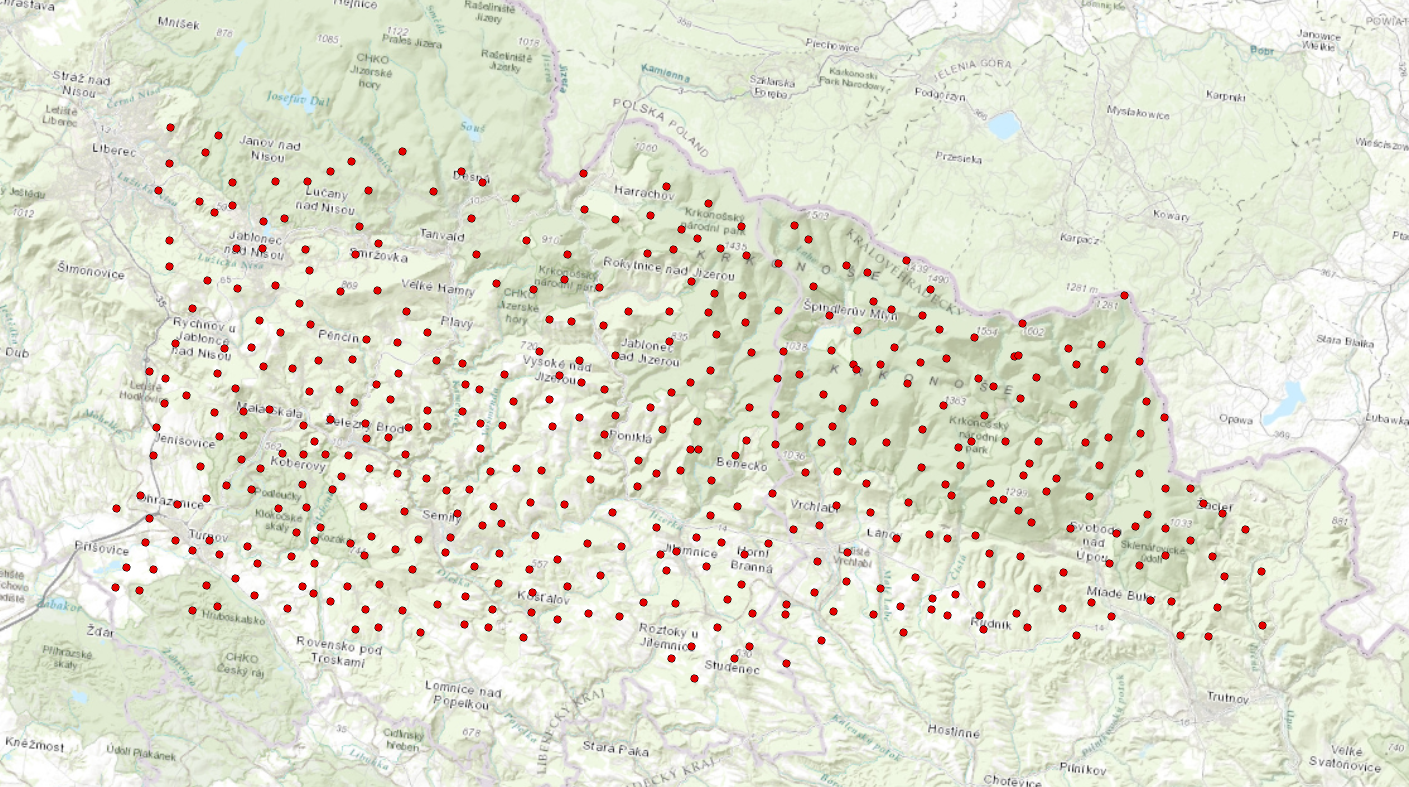
\includegraphics[width=15cm]{images/krkonose2.png} 
    \caption{Vymezení trigonometrických bodů na podkladové mapě.}
\end{figure}
\bigbreak
\par {\large\textbf{Případ 1: Oblast s malou vertikální členitostí} }
\par První zájmovou oblast zobrazuje obr. 11 v šesti oknech. Rozmístění bodů na podkladové mapě se nachází v okně (a), z čehož je zřejmé, že severní část oblasti je jen velmi málo členitá, vertikální členitost pak hlavně roste směrem na jihovýchod. Vygenerované vrstevnice s krokem 5 m, 10 m a 20 m jsou zobrazeny v oknech (b), (d), (f). Vrstevnice v rovinaté části odpovídají skutečnému průběhu terénu, s rostoucí nadmořskou výškou směrem na jihovýchod je pak správně naznačena změna členitosti s vyšší hustotou vrstevnic. Vrstevnice v nejjižnější části oblasti však zřejmě nejsou interpolovány správně, co je způsobeno tím, že zájmová oblast se nachází na okraji datasetu, pro který chybí další údaje o průběhu terénu. Je však zřejmé, že pro postačující výsledky lineární interpolace chybí množství bodů; jednotlivé segmenty tvořící vrstevnice jsou ostré, čímž dochází ke ztrátě informace o skutečné změně v tvaru reliéfu. 

\begin{figure}[H]

\begin{subfigure}{.475\linewidth}
\centering
  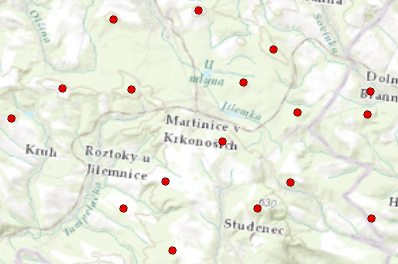
\includegraphics[width=7cm]{images/case1.png}
  \caption{zájmová oblast na podkladové mapě}
  \label{MLEDdet}
\end{subfigure}\hfill % <-- "\hfill"
\begin{subfigure}{.475\linewidth}
\centering
  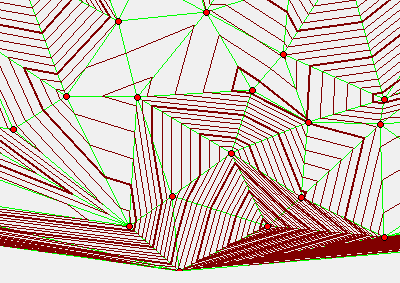
\includegraphics[width=7cm]{images/case1m5.png}
  \caption{vrstevnice s krokem 5 m}
  \label{energydetPSK}
\end{subfigure}\hfill
\medskip
\medskip
\begin{subfigure}{.475\linewidth}
\centering
  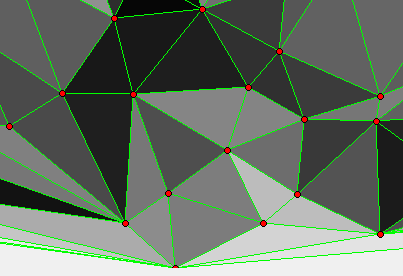
\includegraphics[width=7cm]{images/case1s.png}
  \caption{sklon terénu}
  \label{MLEDdet}
\end{subfigure}\hfill % <-- "\hfill"
\begin{subfigure}{.475\linewidth}
\centering
  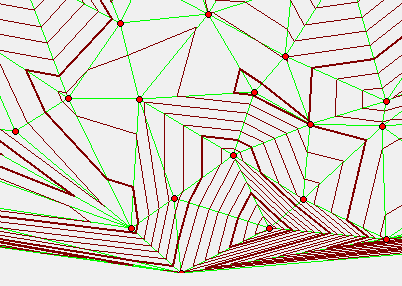
\includegraphics[width=7cm]{images/case1m.png}
  \caption{vrstevnice s krokem 10 m}
  \label{MLEDdet}
\end{subfigure}\hfill % <-- "\hfill"
\medskip
\begin{subfigure}{.475\linewidth}
\centering
  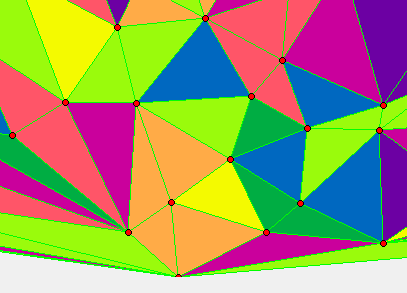
\includegraphics[width=7cm]{images/case1a.png}
  \caption{orientace terénu}
  \label{velcomp}
\end{subfigure}\hfill % <-- "\hfill"
\begin{subfigure}{.475\linewidth}
\centering
  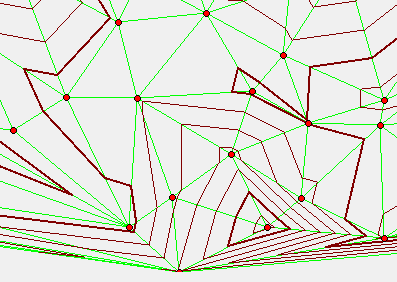
\includegraphics[width=7cm]{images/case1m20.png}
  \caption{vrstevnice s krokem 20 m}
  \label{estcomp}
\end{subfigure}

\caption{Zájmová oblast 1}
\label{fig:roc}
\end{figure}

\par Okno (c) znázorňující sklon svahů odpovídá vygenerovaným vrstevnicím: oblast s tmavými trojúhelníky naznačuje menší členitost, světlejší trojúhelníky naopak vyšší sklon svahu. Opět je důležité upozornit na světlé trojúhelníky v jižní části, které by podle takové analýzy znamenaly vysokou sklonitost terénu. Tento výsledek není správný a souvisí s okrajem analyzovaného území. Orientace svahů v okně (e) pak poukazuje na typy tvarů reliéfu: v jižní části je barevná paleta rozmanitější, což značí různou orientaci svahů kopce, resp. vrcholu, v severní části jsou pak barvy homogennější, protože na rovnějších oblastech nedochází k výrazné změně orientace svahů.
\bigbreak

\par {\large\textbf{Případ 2: Oblast s velkou vertikální členitostí} }
\par Druhá zájmová oblast (obr. 12) se nachází v nejvyšších částech Krkonoš a je charakterizována velkým počtem hřbetů, vrcholů a údolí. Podle vygenerovaných vrstevnic v oknech (b), (d) a (f) je však patrné, že tato oblast nebyla z hlediska výškopisu popsána správně. I když hustota vrstevnic potvrzuje prudkou změnu výškových poměrů, vzhledem k malému počtu bodů vrstevnice nenásledují průběh hřbetů a zcela ignorují většinu údolí. Příčinou je také rozmístění bodů, které v údolích a nižších částech území úplně chybějí a tyto reliéfní tvary tak nemohou být zkonstruovány. Rozmístění bodů také ovlivňuje velikost trojúhelníků, přičemž opět platí, že velké trojúhelníky nemusí dostatečně charakterizovat tvar terénu. Protože je tato oblast opět na okraji datasetu, došlo k nesprávné interpolaci okraje oblasti stejně jako v případě 1.

\begin{figure}[H]

\begin{subfigure}{.475\linewidth}
\centering
  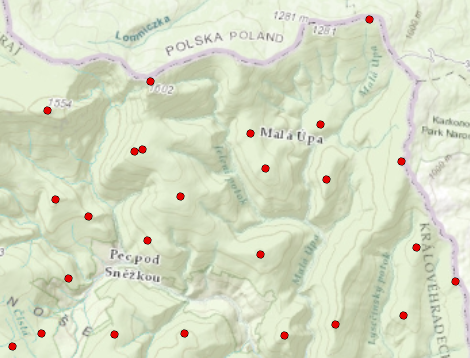
\includegraphics[width=7cm]{images/case2.png}
  \caption{zájmová oblast na podkladové mapě}
  \label{MLEDdet}
\end{subfigure}\hfill % <-- "\hfill"
\begin{subfigure}{.475\linewidth}
\centering
  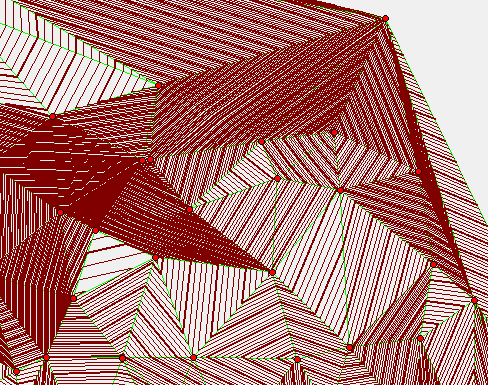
\includegraphics[width=7cm]{images/case2m5.png}
  \caption{vrstevnice s krokem 5 m}
  \label{energydetPSK}
\end{subfigure}\hfill
\medskip
\medskip
\begin{subfigure}{.475\linewidth}
\centering
  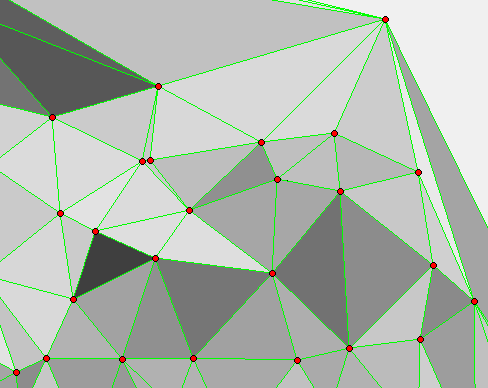
\includegraphics[width=7cm]{images/case2s.png}
  \caption{sklon terénu}
  \label{MLEDdet}
\end{subfigure}\hfill % <-- "\hfill"
\begin{subfigure}{.475\linewidth}
\centering
  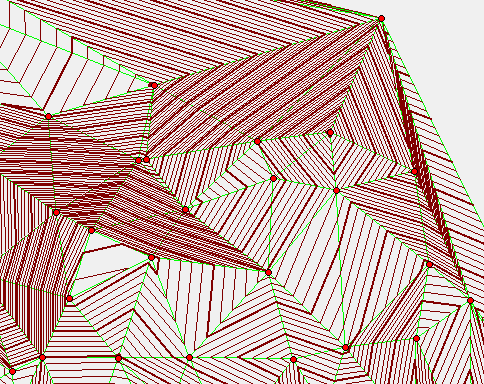
\includegraphics[width=7cm]{images/case2m.png}
  \caption{vrstevnice s krokem 10 m}
  \label{MLEDdet}
\end{subfigure}\hfill % <-- "\hfill"
\medskip
\begin{subfigure}{.475\linewidth}
\centering
  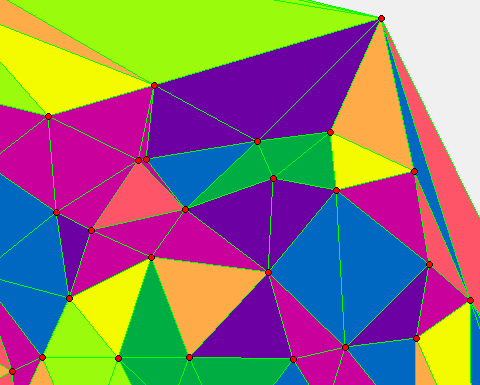
\includegraphics[width=7cm]{images/case2a.png}
  \caption{orientace terénu}
  \label{velcomp}
\end{subfigure}\hfill % <-- "\hfill"
\begin{subfigure}{.475\linewidth}
\centering
  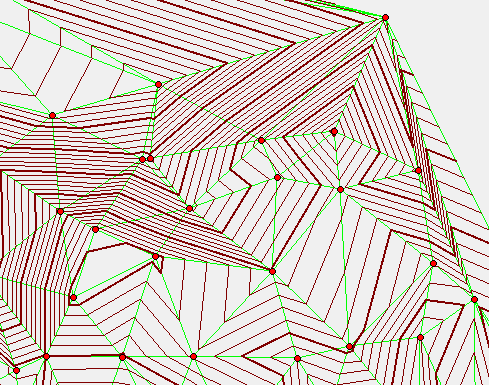
\includegraphics[width=7cm]{images/case2m20.png}
  \caption{vrstevnice s krokem 20 m}
  \label{estcomp}
\end{subfigure}

\caption{Zájmová oblast 2}
\label{fig:roc}
\end{figure}

\par Další zajímavou chybu v modelu odhaluje okno (c) se sklonem terénu, kde je možné pozorovat tmavý trojúhelník v západní části oblasti uprostřed prudkých svahů, což naznačuje rovinatou oblast. Není tomu tak, v skutečnosti vrcholy tohoto trojúhelníku tvoří vrcholy s podobnými nadmořskými výškami a zcela opomíjejí údolí, nad kterým se vypínají. Světlost většiny trojúhelníků však potvrzuje, že se jedná o horskou oblast. Orientaci terénu v okně (e) ovlivňuje nadmořská výška nejvyššího z vrcholů trojúhelníku, a tedy na některých místech, kde dochází k opomenutí reliefních tvarů, je orientace terénu vůči světovým stranám určena nesprávně.
\bigbreak
\par {\large\textbf{Případ 3: oblast s hřebenem a údolími} }
\par Poslední ukázka se věnuje oblasti v severozápadní části analyzovaných dat. Detail oblasti i s grafickými výsledky jsou k dispozici na Obrázku 13. 

\begin{figure}[H]

\begin{subfigure}{.475\linewidth}
\centering
  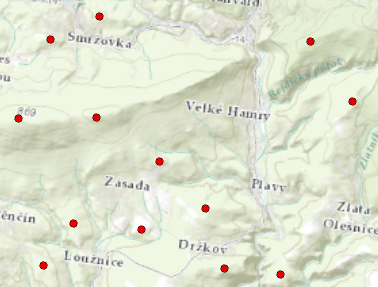
\includegraphics[width=7cm]{images/case3.png}
  \caption{zájmová oblast na podkladové mapě}
  \label{MLEDdet}
\end{subfigure}\hfill % <-- "\hfill"
\begin{subfigure}{.475\linewidth}
\centering
  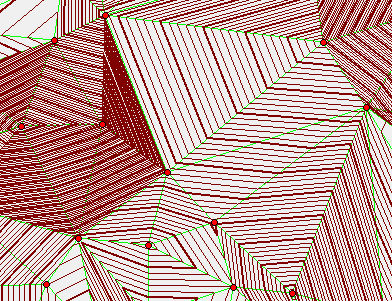
\includegraphics[width=7cm]{images/case3m5.png}
  \caption{vrstevnice s krokem 5 m}
  \label{energydetPSK}
\end{subfigure}\hfill
\medskip
\medskip
\begin{subfigure}{.475\linewidth}
\centering
  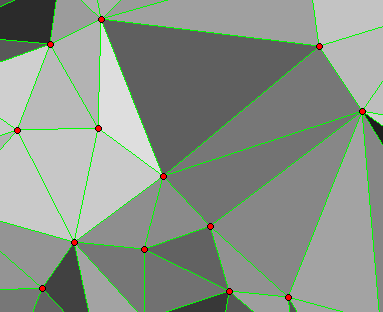
\includegraphics[width=7cm]{images/case3s.png}
  \caption{sklon terénu}
  \label{MLEDdet}
\end{subfigure}\hfill % <-- "\hfill"
\begin{subfigure}{.475\linewidth}
\centering
  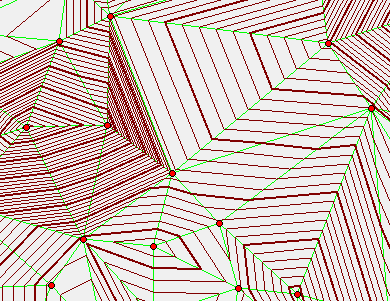
\includegraphics[width=7cm]{images/case3m.png}
  \caption{vrstevnice s krokem 10 m}
  \label{MLEDdet}
\end{subfigure}\hfill % <-- "\hfill"
\medskip
\begin{subfigure}{.475\linewidth}
\centering
  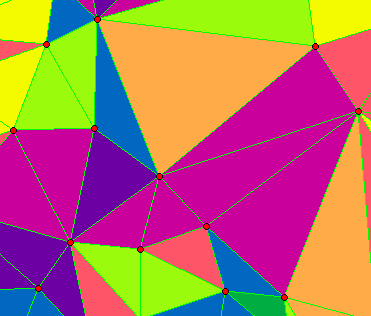
\includegraphics[width=7cm]{images/case3a.png}
  \caption{orientace terénu}
  \label{velcomp}
\end{subfigure}\hfill % <-- "\hfill"
\begin{subfigure}{.475\linewidth}
\centering
  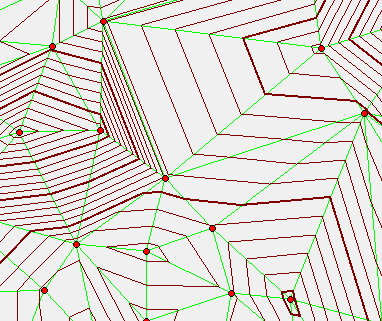
\includegraphics[width=7cm]{images/case3m20.png}
  \caption{vrstevnice s krokem 20 m}
  \label{estcomp}
\end{subfigure}

\caption{Zájmová oblast 3}
\label{fig:roc}
\end{figure}

\par Tato oblast může při grafickém znázornění vrstevnic na první pohled rychle zaujmout: určité trojúhelníky hustěji vyplněny vrstevnicemi díky rychlému nárůstu výšky. Pokud výsledek srovnáme s realitou, tak je patrné, že vzniklá triangulace v okolí dvou bodů na hřebenu (na obrázku (a) se nacházejí na v západní části) proběhla až na malé odlišnosti dobře. Ovšem tento hřeben pokračuje směrem na východ (severovýchod), což výsledek vizualizovaných vrstevnic nerespektuje. Tato skutečnost, jak již bylo zmíněno, vyplývá z faktu, že algoritmus, který je použitý pro výpočet triangulace, nerespektuje žádné překážky jako vodní toky nebo silnice. Hřeben by měl pokračovat dál na východ, který se mírně svažuje a následně je přerušen údolím. Na druhý pohled je však z výsledků vygenerovaných vrstevnic vidět jakýsi náznak údolí, které ovšem prochází středem sledované zájmové oblasti. Lze tedy říci, že pokud bychom měli k dispozici více bodů z terénu, nebo by bylo do výpočtu zahrnuto respektování bariér (řeky,\dots) výsledek triangulace by více odpovídal skutečnosti. Pokud se budeme soustředit na expozici svahu v okolí těchto bodů (e) zjistíme, že výsledek odpovídá skutečnosti a lze tedy potvrdit, že implementovaný algoritmus pro analýzu orientace svahu pracuje správně.
\par Uprostřed jižní části výřezu se nachází bod, který dle výsledné triangulace a i vzhledem k realitě reprezentuje vrchol kopce. Ovšem ve skutečnosti se směrem na jih/jihovýchod nachází rovina, kterou algoritmus nemá šanci (vzhledem k datům) rozpoznat. Opět lze tedy konstatovat, že nad analyzovanými daty je zanedbaná důležitá informace o průběhu terénu. V této části zájmového území neodpovídá analýza sklonu ani orientace terénu skutečnosti. Pokud bychom ovšem nahlíželi na území jen z hlediska výšky, pak je výsledná analýza provedená správně.

\bigbreak
\par {\large\textbf{Shrnutí} }
\par Implementované metody pro konstrukci a analýzu DMT byly otestovány na členitém reliéfu Krkonoš s nereprezentativním vzorkem dat. I přestože byly určité části území popsány z hlediska výškopisu, svažitosti a orientace svahů vůči světovým stranám správně, není možné ohodnotit celkový výsledek analýzy vytvořeného modelu kladně. Jako hlavní příčiny byly identifikovány následující skutečnosti:
\begin{itemize}
    \item nedostatečný počet bodů v datasetu, a tedy menší počet trojúhelníků na místech, kde se tvar reliéfu mění intenzivněji,
    \item nevhodné rozmístění bodů, které se nacházejí téměř výhradně na vrcholech pohoří a na níže položených místech území zcela chybějí,
    \item využití lineární interpolace, která není pro náročnější terén vhodná a je vhodné ji doplnit jinými technikami/metodami.
\end{itemize}

\par Bylo by vhodné provést konstrukci a analýzu DMT nad jiným datasetem, který by zohledňoval výše popsané nedostatky.


\chapter*{Závěr}

\par V této úloze byly představeny a implementovány algoritmy \emph{Ray Crossing} a \emph{Winding Number}, které jsou schopny řešit \emph{Point-in-Polygon Problem} pro nekonvexní útvary. Jejich funkčnost byla testována pomocí vytvorěné aplikace, která umožňuje provést analýzu polohy bodu vůči zvolené polygonové mapě ve formátu \verb|JSON| nebo \verb|GeoJSON|. Tato aplikace byla vytvořena v programovacím jazyce \verb|Python 3.11|.
\par Samotnou aplikaci je možné vylepšit o přidání podpory pro jiné formáty obsahující prostorovou informaci (napr. \verb|shapefile|). Současný stav aplikace navíc neumožňuje načíst \verb|JSON| a \verb|GeoJSON| soubory v jiném než nestardandním formátu – je nutno zabezpečit nalezení souřadnic v různě uspořádaných slovnících a seznamech v \verb|JSON|u a \verb|GeoJSON|u. Další možné vylepšení je implementace dynamické měnění velikosti načteného obsahu vzhledem k velikosti okna. Vhodným doplňkem může být i možnost přiblížení/oddálení obsahu okna pro zpřesnení umístění bodu.
\par Vytvořená aplikace je volně dostupná přes \verb|GitHub| na adrese \url{https://github.com/koziskoa/APK_2023/tree/master/point_in_polygon}.
\begin{thebibliography}{9}
\bibitem{Bayer 2008}
BAYER, T. (2008): Algoritmy v digitální kartografii. Nakladatelství Karolinum, Praha.

\bibitem{Bayer 2023}
BAYER, T. (2023): Point Location Problem. Přednáška pro předmět Algoritmy počítačové kartografie, Katedra aplikované geoinformatiky a kartografie. Přírodověděcká fakulta UK, dostupné \href{http://web.natur.cuni.cz/~bayertom/images/courses/Adk/adk3_new.pdf}{\emph{zde}} (cit. 13. 3. 2023).

\bibitem{Rouke}
ROURKE, O. J. (2005): Computational Geometry in C. Cambridge University Press, Cambridge.

\bibitem{Zara}
ŽÁRA, J., BEDŘICH, B., SOCHOR, J., FELKEL, P. (2004): Moderní počítačová grafika. Computer Press, Brno.
\end{thebibliography}

\end{document}

